%! Unidad 11 — Dinámica aplicada: interacción gravitatoria y electrostática, fuerzas de contacto, dinámica del movimiento
%! rectilíneo (planos horizontales e inclinados, cuerpos enlazados) y del movimiento circular
%! (teoría, ejemplos resueltos, ejercicios por apartados, lectura, prácticas y situación de aprendizaje)
%! Fuente: Fuentes/Fisica/Unidad 11 (capturas 425 —portada, mitad derecha— y 426-438, solucionario) y Unidad 12 (captura 439:
%!   olimpiadas y autoevaluación de este tema).
%! Texto reescrito; datos de los ejercicios cambiados (y más realistas cuando los de la fuente no lo eran) y recalculados; g = 9,8 m/s².
%! Figuras en images/UD11/: nuevas en html/ (cuerpos_enlazados, curvas, practica_libro), copiadas (PDF + SVG) de 4ESO/images/UD9
%!   (gravitacion, orbitas_satelites, sin_fuerza_centripeta), de 4ESO/images/UD8 (fuerzas_cuerpos) y de 2BachFisica/images/UD5
%!   (coulomb, electrizacion). Reutiliza images/UD10/plano_inclinado. Gráfica de la fuerza de rozamiento con pgfplots.

\section*{Para empezar: ¿física de película?}
\addcontentsline{toc}{section}{Para empezar: ¿física de película?}

Persecuciones de vértigo, explosiones, rescates imposibles, batallas entre naves espaciales\dots\ El cine nos ofrece escenas
espectaculares, pero ¿respetan las leyes de la física? Algunas producciones cuentan con asesores científicos y cuidan mucho los
detalles; otras sacrifican la física por el espectáculo. Con lo que vamos a aprender en esta unidad podrás mirar con ojo crítico
películas como \textit{Interstellar}, \textit{Star Wars} o las de superhéroes.

En la unidad anterior establecimos las leyes de Newton. Ahora las aplicaremos a situaciones concretas: conoceremos las fuerzas más
habituales (el peso, la fuerza eléctrica, la normal, el rozamiento, la tensión y la fuerza elástica) y aprenderemos a resolver
problemas de cuerpos en planos horizontales e inclinados, de cuerpos enlazados y de movimientos circulares.

%========================================================================================
\section{Recuerda de la ESO}\label{sec:ud11-eso}
%========================================================================================

\paragraph{Fuerzas a distancia y de contacto.} Las fuerzas \textbf{a distancia} no necesitan que los cuerpos se toquen (la atracción
entre la Tierra y la Luna, entre dos cargas o entre dos imanes); las fuerzas \textbf{de contacto} sí (empujar un carrito, el rozamiento
entre dos superficies).

\paragraph{Segunda ley de Newton.} La resultante de las fuerzas exteriores que actúan sobre un cuerpo es igual a su masa por su
aceleración: \(\sum \vec{F} = m\,\vec{a}\). Será la herramienta con la que resolveremos todos los problemas de la unidad.

\paragraph{El peso.} Es la fuerza con que la Tierra atrae a un cuerpo. Tiene la dirección de la vertical del lugar (la que marca una
plomada), sentido hacia el centro de la Tierra y módulo \(P = m\,g\), con \(g = \qty{9.8}{\m\per\s\squared}\) en la superficie terrestre.

\paragraph{La normal, la tensión y el rozamiento.} La \textbf{normal}, \(\vec{N}\), es la fuerza que hace una superficie sobre un cuerpo
apoyado en ella, siempre perpendicular a la superficie. La \textbf{tensión}, \(\vec{T}\), es la fuerza que transmite una cuerda tensa. La
\textbf{fuerza de rozamiento}, \(\vec{F}_r\), se opone al deslizamiento de una superficie sobre otra; se debe a las irregularidades de
las superficies y vale \(F_r = \mu\,N\), donde \(\mu\) es el \textbf{coeficiente de rozamiento}, que depende de los dos materiales.

\paragraph{Carga eléctrica.} Es una propiedad de la materia: los protones tienen carga positiva y los electrones, negativa. La carga
de un cuerpo es siempre un múltiplo entero de la carga elemental, \(q = z\,e\), con \(e = \qty{1.6e-19}{\coulomb}\). Un cuerpo neutro
puede \textbf{electrizarse} por frotamiento, por contacto o por inducción (figura~\ref{fig:ud11-electrizacion}).

\begin{figure}[H]
    \centering
    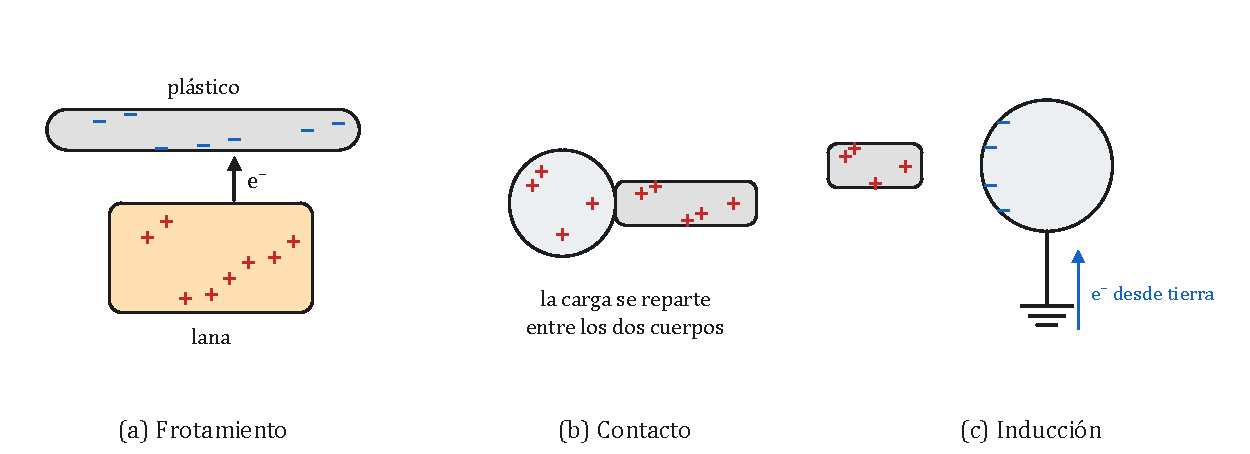
\includegraphics[width=0.8\textwidth]{images/UD11/electrizacion}
    \caption{Formas de electrizar un cuerpo: por frotamiento, por contacto y por inducción.}
    \label{fig:ud11-electrizacion}
\end{figure}

\begin{exercise}
    Un objeto de plástico frotado con un paño adquiere una carga de \qty{-3.2}{\nano\coulomb}. a) ¿Ha ganado o ha perdido electrones?
    ¿Cuántos? b) ¿Qué carga ha adquirido el paño?
    \begin{solu}
        a) \textcolor{red}{Ha ganado} \(\dfrac{\num{3.2e-9}}{\num{1.6e-19}} = \textcolor{red}{\num{2e10}~\text{electrones}}\).
        b) \textcolor{red}{\qty{+3.2}{\nano\coulomb}}: la carga se conserva, y el paño ha perdido esos electrones.
    \end{solu}
\end{exercise}

%========================================================================================
\section{Cómo se resuelve un problema de dinámica}\label{sec:ud11-esquema}
%========================================================================================

La segunda ley de Newton, \(\vec{F}_{\text{neta}} = m\,\vec{a}\), nos permite estudiar la evolución de un objeto en multitud de
situaciones. Para aplicarla bien hay que tener en cuenta dos cosas:

\begin{itemize}
    \item Es una ecuación \textbf{vectorial}, que equivale a una ecuación para cada componente:
    \(\sum F_x = m\,a_x\) y \(\sum F_y = m\,a_y\).
    \item Hay que \textbf{identificar bien todas las fuerzas} que actúan sobre el cuerpo: qué otro cuerpo las ejerce, en qué dirección
    actúan y cuánto valen.
\end{itemize}

\begin{definition}[Procedimiento para resolver un problema de dinámica]
    \textbf{1.}~\textbf{Representa el cuerpo} como un punto o una caja: no nos interesan su forma ni su tamaño, sino el movimiento de su
        centro de masas.

    \textbf{2.}~\textbf{Identifica y dibuja todas las fuerzas} que actúan sobre él (¿lo atrae otro cuerpo? ¿está apoyado? ¿hay rozamiento?
        ¿está unido a cuerdas o muelles?). Este dibujo se llama \textbf{diagrama de cuerpo libre}.

    \textbf{3.}~\textbf{Elige un sistema de referencia}, con un eje en la dirección del movimiento, y \textbf{descompón} las fuerzas que no
        estén sobre los ejes.

    \textbf{4.}~\textbf{Aplica la segunda ley de Newton} a cada eje y resuelve las ecuaciones.
\end{definition}

\begin{remark}
    Aunque se cumpla la tercera ley de Newton, en el diagrama solo se dibujan las fuerzas que actúan \textbf{sobre} el cuerpo que
    estudiamos, no las que él ejerce sobre otros. Si hay varios cuerpos, se dibuja un diagrama para cada uno y se plantean sus
    ecuaciones por separado.
\end{remark}

\begin{figure}[H]
    \centering
    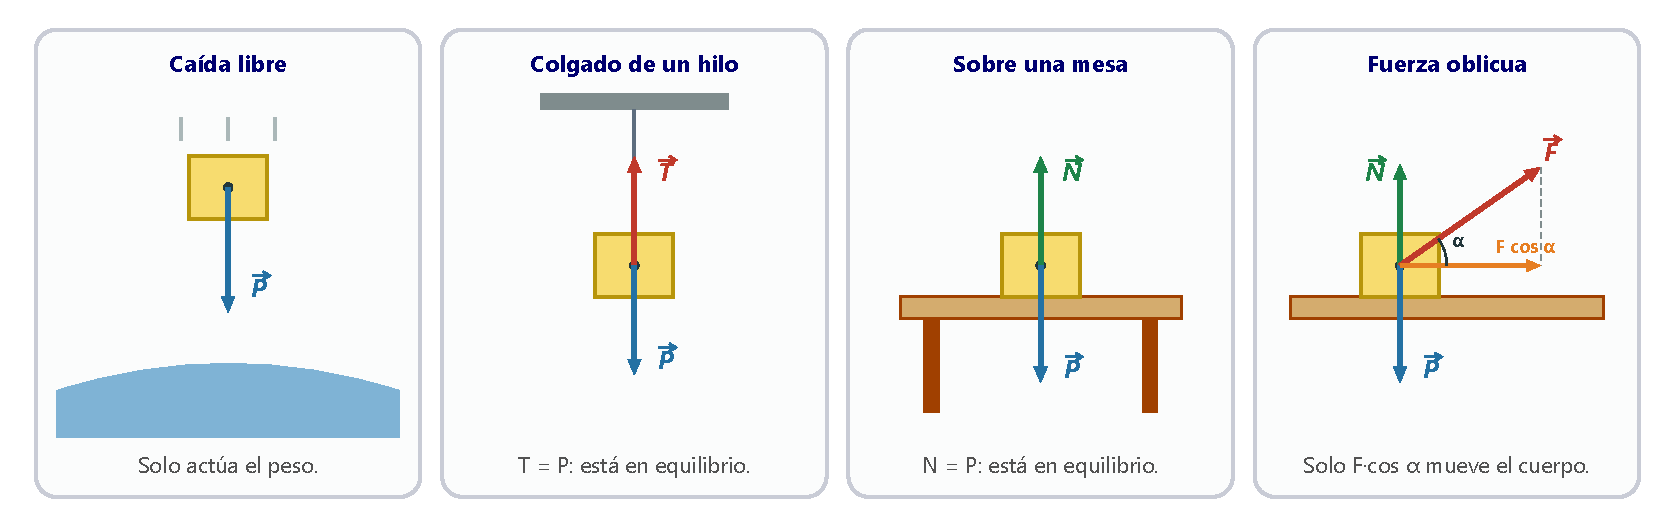
\includegraphics[width=\textwidth]{images/UD11/fuerzas_cuerpos}
    \caption{Diagramas de cuerpo libre de un cuerpo en algunas situaciones sencillas.}
    \label{fig:ud11-diagramas}
\end{figure}

%========================================================================================
\section{La interacción gravitatoria y el peso}\label{sec:ud11-gravitatoria}
%========================================================================================

\subsection{Ley de la gravitación universal}

Newton propuso en 1687, a partir de los trabajos de Kepler y de sus propias medidas, que todos los cuerpos se atraen por el simple
hecho de tener masa.

\begin{definition}[Ley de la gravitación universal]
    Dos cuerpos se atraen con una fuerza directamente proporcional al producto de sus masas e inversamente proporcional al cuadrado
    de la distancia que los separa:
    \[ F = G\,\frac{m_1\,m_2}{r^2} \qquad G = \qty{6.67e-11}{\newton\m\squared\per\kg\squared} \]
\end{definition}

\begin{itemize}
    \item La fuerza tiene la dirección de la recta que une los dos cuerpos y es siempre \textbf{atractiva}. Por la tercera ley de
    Newton, cada cuerpo atrae al otro con una fuerza del mismo módulo (figura~\ref{fig:ud11-gravitacion}).
    \item La \textbf{constante de gravitación universal}, \(G\), tiene el mismo valor en todo el universo. Es tan pequeña que solo los
    cuerpos de masa enorme, como los planetas, ejercen fuerzas gravitatorias apreciables.
\end{itemize}

\begin{figure}[H]
    \centering
    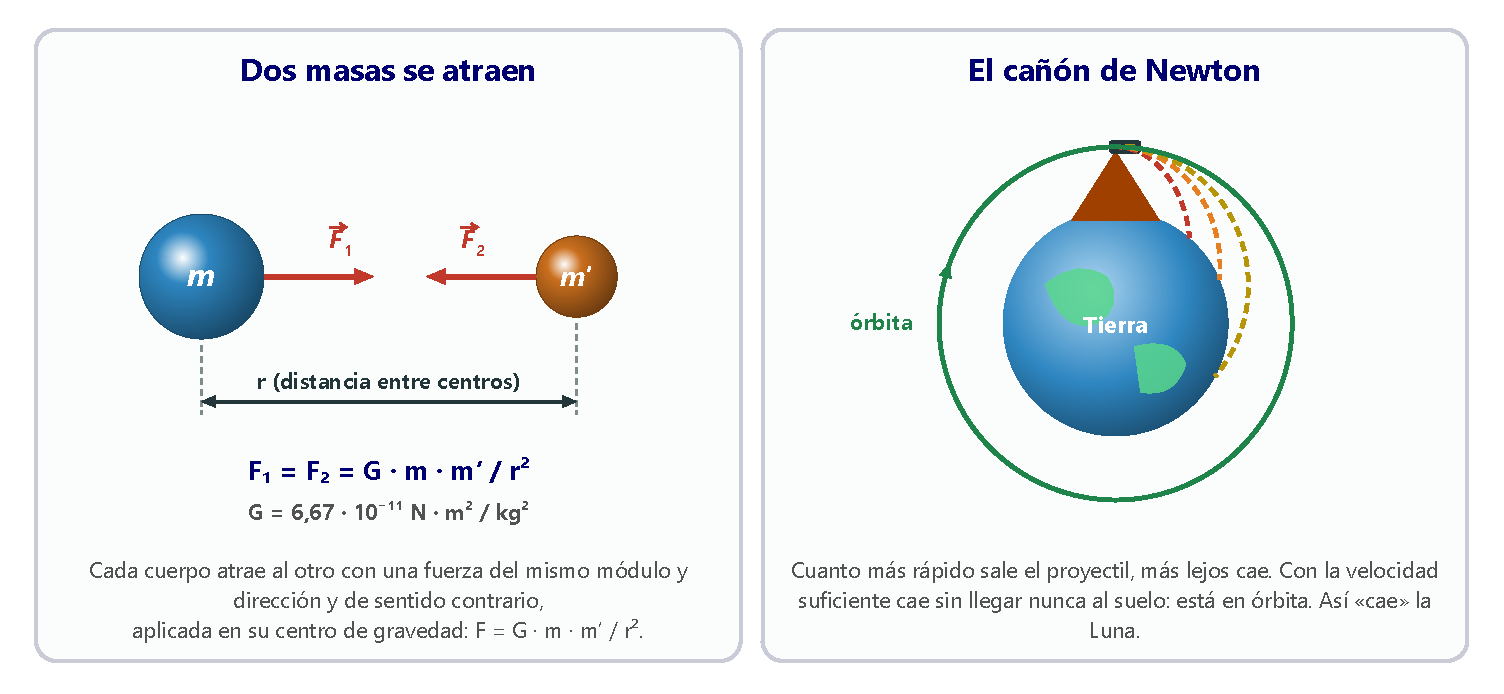
\includegraphics[width=0.55\textwidth]{images/UD11/gravitacion}
    \caption{Dos masas se atraen con fuerzas iguales y opuestas.}
    \label{fig:ud11-gravitacion}
\end{figure}

\subsection{El peso de los cuerpos}

El peso es un caso particular de la ley de la gravitación universal: es la fuerza con que la Tierra, de masa \(M_T\) y radio \(R_T\),
atrae a los cuerpos situados en su superficie:
\[ P = G\,\frac{M_T\,m}{R_T^2} = m\,g \qquad \text{con} \qquad g = G\,\frac{M_T}{R_T^2} = \qty{9.8}{\m\per\s\squared} \]

\begin{itemize}
    \item \textbf{Módulo}: \(P = m\,g\). \textbf{Dirección}: radial, la de la recta que une el cuerpo con el centro de la Tierra.
    \textbf{Sentido}: hacia el centro de la Tierra. \textbf{Punto de aplicación}: el centro de gravedad del cuerpo.
    \item El peso depende de la distancia al centro de la Tierra. La expresión \(P = m\,g\) con \(g = \qty{9.8}{\m\per\s\squared}\) solo
    vale cerca de la superficie, cuando la altura es pequeña comparada con el radio terrestre.
    \item En otros astros, \(g\) es distinta porque depende de su masa y de su radio. La masa de un astronauta es la misma en la Tierra
    y en la Luna, pero en la Luna, donde \(g = \qty{1.62}{\m\per\s\squared}\), pesa unas seis veces menos.
\end{itemize}

\begin{example}
    \textbf{El peso en la Estación Espacial.} ¿Cuánto pesa una astronauta de \qty{70}{\kg} en la Estación Espacial Internacional, a
    \qty{408}{\km} de altura? Compáralo con su peso en la superficie. (\(M_T = \qty{5.97e24}{\kg}\), \(R_T = \qty{6370}{\km}\).)

    \textbf{Solución.} La distancia al centro de la Tierra es \(r = 6370 + 408 = \qty{6778}{\km}\):
    \[ P = G\,\frac{M_T\,m}{r^2} = \num{6.67e-11} \cdot \frac{\num{5.97e24} \cdot 70}{(\num{6.778e6})^2} = \qty{607}{\newton} \]
    En la superficie pesaría \(70 \cdot \num{9.8} = \qty{686}{\newton}\): en la Estación pesa \textbf{un 88\,\%} de su peso habitual. Si
    los astronautas flotan no es porque no pesen, sino porque la Estación y todo lo que hay dentro caen juntos alrededor de la Tierra.
\end{example}

\begin{exercise}
    Calcula el peso de una persona de \qty{80}{\kg} en la Tierra, en la Luna, en Marte y en Venus. (\(g_L = \qty{1.62}{\m\per\s\squared}\);
    \(g_M = \qty{3.71}{\m\per\s\squared}\); \(g_V = \qty{8.87}{\m\per\s\squared}\).)
    \begin{solu}
        \textcolor{red}{Tierra: \qty{784}{\newton}; Luna: \qty{130}{\newton}; Marte: \qty{297}{\newton}; Venus: \qty{710}{\newton}.}
    \end{solu}
\end{exercise}

\begin{exercise}
    Una persona pesa \qty{130}{\newton} en la Luna. ¿Cuál es su masa? ¿Cuánto pesará en la Tierra?
    \begin{solu}
        \(m = \dfrac{130}{\num{1.62}} = \textcolor{red}{\qty{80.2}{\kg}}\); \(P_T = \num{80.2} \cdot \num{9.8} = \textcolor{red}{\qty{786}{\newton}}\).
    \end{solu}
\end{exercise}

%========================================================================================
\section{La interacción electrostática}\label{sec:ud11-electrostatica}
%========================================================================================

Frota un bolígrafo de plástico con un jersey de lana y acércalo a unos trocitos de papel: los atrae. Ya hacia el año 600 a.\,C., Tales
de Mileto observó que el ámbar frotado atraía objetos ligeros; de ahí viene la palabra \textit{electricidad}, del griego
\textit{elektron}, «ámbar». Las fuerzas entre cargas en reposo se llaman \textbf{electrostáticas}.

\begin{definition}[Ley de Coulomb]
    La fuerza entre dos cargas puntuales es directamente proporcional al producto de las cargas e inversamente proporcional al
    cuadrado de la distancia que las separa:
    \[ F = k\,\frac{|q_1\,q_2|}{r^2} \]
    En el vacío, \(k = \qty{9e9}{\newton\m\squared\per\coulomb\squared}\).
\end{definition}

Charles-Augustin de Coulomb la estableció en 1785 midiendo fuerzas con una balanza de torsión. Sus características son:
\begin{itemize}
    \item La fuerza tiene la dirección de la recta que une las cargas.
    \item A diferencia de la gravitatoria, puede ser \textbf{atractiva o repulsiva}: las cargas de distinto signo se atraen y las del
    mismo signo se repelen (figura~\ref{fig:ud11-coulomb}).
    \item La constante \(k\) depende del medio en que estén las cargas; en el agua, por ejemplo, es unas 80 veces menor que en el vacío.
    \item Las fuerzas electrostáticas también cumplen la tercera ley de Newton.
\end{itemize}

\begin{figure}[H]
    \centering
    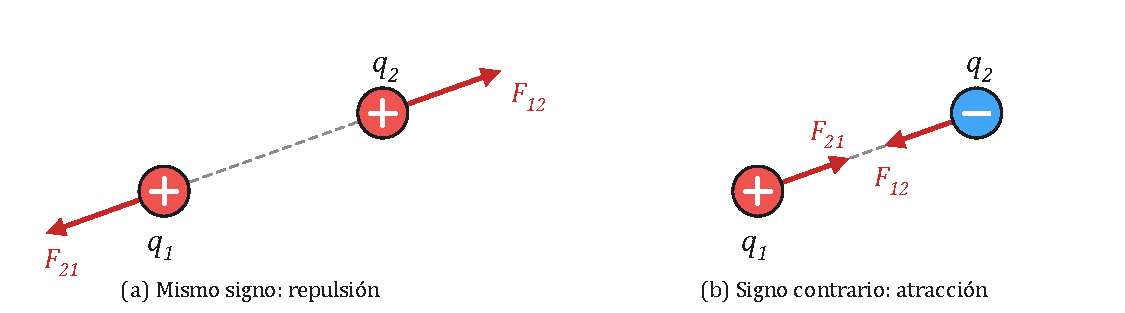
\includegraphics[width=0.75\textwidth]{images/UD11/coulomb}
    \caption{Fuerzas entre dos cargas: repulsión si tienen el mismo signo y atracción si tienen signos contrarios.}
    \label{fig:ud11-coulomb}
\end{figure}

\begin{example}
    \textbf{Fuerza eléctrica y fuerza gravitatoria entre dos iones.} En un cristal de sal común, un ion \ch{Na+} y un ion \ch{Cl-}
    están separados \qty{2.82e-10}{\m}. Calcula la fuerza electrostática y la gravitatoria entre ellos y compáralas. (Masas: \ch{Na}
    \qty{23}{\uma}, \ch{Cl} \qty{35.5}{\uma}; \(\qty{1}{\uma} = \qty{1.66e-27}{\kg}\).)

    \textbf{Solución.} Cada ion tiene una carga elemental, \(\num{1.6e-19}\)~C:
    \[ F_e = k\,\frac{|q_1\,q_2|}{r^2} = \num{9e9} \cdot \frac{(\num{1.6e-19})^2}{(\num{2.82e-10})^2} = \qty{2.9e-9}{\newton} \]
    \[ F_g = G\,\frac{m_1\,m_2}{r^2} = \num{6.67e-11} \cdot \frac{(23 \cdot \num{1.66e-27}) \cdot (\num{35.5} \cdot \num{1.66e-27})}{(\num{2.82e-10})^2}
    = \qty{1.9e-42}{\newton} \]
    La fuerza eléctrica es unas \(\num{1.5e33}\) veces mayor: en el mundo de los átomos la gravedad es completamente despreciable, y
    los enlaces químicos son de naturaleza eléctrica.
\end{example}

\begin{exercise}
    Calcula la fuerza con que se repelen dos bolitas con una carga de \qty{+3}{\micro\coulomb} cada una si están separadas
    \qty{15}{\cm}. Representa la fuerza sobre cada carga.
    \begin{solu}
        \(F = \num{9e9} \cdot \dfrac{(\num{3e-6})^2}{\num{0.15}^2} = \textcolor{red}{\qty{3.6}{\newton}}\), en la recta que las une y
        \textcolor{red}{alejando cada carga de la otra}.
    \end{solu}
\end{exercise}

\begin{exercise}
    ¿A qué distancia deben estar dos cargas de \qty{+20}{\nano\coulomb} y \qty{-20}{\nano\coulomb} para atraerse con una fuerza de
    \qty{0.3}{\newton}?
    \begin{solu}
        \(r = \sqrt{\dfrac{\num{9e9} \cdot (\num{2e-8})^2}{\num{0.3}}} = \textcolor{red}{\qty{3.5e-3}{\m}}\) (\qty{3.5}{\mm}).
    \end{solu}
\end{exercise}

%========================================================================================
\section{Fuerzas de contacto}\label{sec:ud11-contacto}
%========================================================================================

Las fuerzas de contacto solo actúan mientras los cuerpos se tocan: cuando cesa el contacto, cesa la interacción. Por eso, una vez
lanzada una pelota, la fuerza de la mano ya no actúa sobre ella. Aunque parezcan muy distintas, todas estas fuerzas se deben, a escala
microscópica, a interacciones electromagnéticas entre los átomos de las superficies.

\subsection{La fuerza normal}

Un libro apoyado en la mesa no la atraviesa ni cae, aunque la Tierra lo atrae. Si está en equilibrio, alguna fuerza compensa su peso:
la que le hace la mesa.

\begin{definition}[Fuerza normal]
    Es la fuerza que ejerce una superficie sobre un cuerpo apoyado en ella. Es la reacción de la superficie a la fuerza con que el
    cuerpo la presiona.
\end{definition}

\begin{itemize}
    \item Es siempre \textbf{perpendicular a la superficie de apoyo} y dirigida hacia fuera de ella.
    \item Su módulo \textbf{depende de las demás fuerzas} que actúan sobre el cuerpo: se obtiene aplicando la segunda ley en la
    dirección perpendicular a la superficie. No siempre es igual al peso.
    \item La normal \textbf{no es la reacción del peso}: el peso es una interacción Tierra-cuerpo y la normal, una interacción
    superficie-cuerpo.
    \item Solo hay normal si hay apoyo: si un cuerpo toca una superficie pero no la presiona, la normal es nula.
\end{itemize}

\begin{example}
    \textbf{Presionar un libro.} Empujamos hacia abajo con una fuerza de \qty{12}{\newton} un libro de \qty{1.5}{\kg} apoyado en una
    mesa. ¿Cuánto vale la normal?

    \textbf{Solución.} Sobre el libro actúan su peso y nuestra fuerza (hacia abajo) y la normal (hacia arriba). Está en equilibrio:
    \[ N - P - F = 0 \Rightarrow N = \num{1.5} \cdot \num{9.8} + 12 = \qty{26.7}{\newton} \]
\end{example}

\begin{exercise}
    Un bloque de \qty{3}{\kg} está sobre un plano inclinado \(25^\circ\). ¿Cuánto vale la fuerza normal?
    \begin{solu}
        \(N = P_y = 3 \cdot \num{9.8} \cdot \cos 25^\circ = \textcolor{red}{\qty{26.6}{\newton}}\).
    \end{solu}
\end{exercise}

\subsection{Fuerzas de rozamiento}

El rozamiento se debe a las \textbf{irregularidades} de las superficies, que encajan unas con otras, y a las fuerzas de adhesión entre
sus átomos. Siempre se \textbf{opone al movimiento relativo} de un cuerpo respecto a otro.

\begin{definition}[Fuerza de rozamiento]
    Es una fuerza paralela a la superficie de contacto entre dos cuerpos que se opone al deslizamiento de uno respecto al otro.
\end{definition}

\paragraph{Rozamiento estático.} Si intentamos arrastrar un mueble pesado empujando poco a poco con más fuerza, al principio no se
mueve: el rozamiento \textbf{estático} iguala a la fuerza aplicada. Su valor no es fijo: crece con la fuerza aplicada hasta un
\textbf{valor máximo}
\[ F_{re,\,\text{máx}} = \mu_e\,N \]
donde \(\mu_e\) es el \textbf{coeficiente de rozamiento estático}. Solo cuando la fuerza aplicada supera ese máximo el cuerpo empieza
a moverse.

\paragraph{Rozamiento cinético.} Una vez en movimiento, sobre el cuerpo actúa el rozamiento \textbf{cinético} (o dinámico):
\[ F_{rc} = \mu_c\,N \]
donde \(\mu_c\) es el \textbf{coeficiente de rozamiento cinético}. Consideraremos que su valor es constante y no depende de la velocidad.

\begin{figure}[H]
    \centering
    \begin{tikzpicture}
        \begin{axis}[grafica, width=0.55\linewidth, height=5cm, xlabel={Fuerza aplicada, \(F\)}, ylabel={\(F_r\)}, xmin=0, xmax=10,
            ymin=0, ymax=6, xtick={5}, xticklabels={\(\mu_e N\)}, ytick={3.6,5}, yticklabels={\(\mu_c N\),\(\mu_e N\)}]
            \addplot[very thick, ocre, domain=0:5] {x};
            \addplot[very thick, ocre, domain=5:10] {3.6};
            \addplot[dashed, gray] coordinates {(5,5) (5,3.6)};
            \node[font=\scriptsize, align=center] at (axis cs:2.4,4.4) {estático:\\ \(F_r = F\)};
            \node[font=\scriptsize] at (axis cs:7.6,4.2) {cinético};
            \node[font=\scriptsize] at (axis cs:7.6,1.6) {el cuerpo se mueve};
        \end{axis}
    \end{tikzpicture}
    \caption{Fuerza de rozamiento frente a la fuerza aplicada. En reposo, el rozamiento iguala a la fuerza aplicada hasta su valor
    máximo; una vez en movimiento, vale \(\mu_c\,N\), algo menos.}
    \label{fig:ud11-rozamiento}
\end{figure}

\begin{itemize}
    \item Los coeficientes \(\mu_e\) y \(\mu_c\) no tienen unidades y dependen de \textbf{las dos superficies} en contacto
    (tabla~\ref{tab:ud11-coeficientes}), pero apenas dependen del área de contacto.
    \item Normalmente \(\mu_e > \mu_c\): cuesta más poner un cuerpo en movimiento que mantenerlo.
\end{itemize}

\begin{table}[H]
    \centering
    \caption{Valores aproximados de los coeficientes de rozamiento}
    \vspace{-5pt}
    \begin{tabular}{@{}lcc@{}}
        \toprule
        \textbf{Superficies} & \(\boldsymbol{\mu_e}\) & \(\boldsymbol{\mu_c}\) \\
        \midrule
        Madera sobre madera & \num{0.25}-\num{0.5} & \num{0.2} \\[3pt]
        Madera sobre cuero & \num{0.5} & \num{0.4} \\[3pt]
        Acero sobre acero & \num{0.74} & \num{0.57} \\[3pt]
        Neumático sobre asfalto seco & \num{1.0} & \num{0.8} \\[3pt]
        Neumático sobre asfalto mojado & \num{0.7} & \num{0.5} \\[3pt]
        Acero sobre hielo & \num{0.03} & \num{0.01} \\
        \bottomrule
    \end{tabular}
    \label{tab:ud11-coeficientes}
\end{table}

\begin{remark}
    A veces interesa reducir el rozamiento (puliendo las superficies o usando lubricantes, como el aceite de un motor o el líquido
    sinovial de nuestras articulaciones) y otras, aumentarlo (los dibujos de los neumáticos o las suelas de las zapatillas). Sin
    rozamiento no podríamos ni caminar.
\end{remark}

\begin{example}
    \textbf{Arrastrar un cuerpo.} Un cuerpo de \qty{50}{\kg} está en reposo en el suelo. Los coeficientes de rozamiento son
    \(\mu_e = \num{0.45}\) y \(\mu_c = \num{0.30}\). Calcula: a) la fuerza horizontal mínima para ponerlo en movimiento; b) la fuerza de
    rozamiento y la aceleración si se empuja con \qty{300}{\newton}.

    \textbf{Solución.} La normal es igual al peso: \(N = 50 \cdot \num{9.8} = \qty{490}{\newton}\).
    a) \(F_{re,\,\text{máx}} = \mu_e\,N = \num{0.45} \cdot 490 = \qty{220.5}{\newton}\): hay que empujar con algo más de esa fuerza.
    b) Como \(300 > \num{220.5}\), el cuerpo se mueve y el rozamiento es cinético: \(F_r = \num{0.30} \cdot 490 = \qty{147}{\newton}\);
    \(a = \dfrac{300 - 147}{50} = \qty{3.06}{\m\per\s\squared}\).
\end{example}

\begin{exercise}
    Se aprieta un cuerpo de \qty{3}{\kg} contra una pared vertical con una fuerza horizontal de \qty{70}{\newton}. El coeficiente de
    rozamiento estático es \num{0.5}. a) ¿Resbalará? b) ¿Qué fuerza de rozamiento actúa? ¿Qué fuerza hace la pared?
    \begin{solu}
        \textcolor{blue}{\(N = \qty{70}{\newton}\); \(F_{re,\,\text{máx}} = \num{0.5} \cdot 70 = \qty{35}{\newton}\) y \(P = \qty{29.4}{\newton}\).}
        a) \textcolor{red}{No resbala}, porque \(P\) es menor que el rozamiento máximo. b) \(\textcolor{red}{F_r = \qty{29.4}{\newton}}\)
        hacia arriba; la pared hace una normal de \textcolor{red}{\qty{70}{\newton}} (y además el rozamiento).
    \end{solu}
\end{exercise}

\begin{exercise}
    Para mover una lavadora de \qty{50}{\kg} por el suelo de la cocina hay que empujarla con \qty{240}{\newton} antes de que empiece
    a deslizar. a) Calcula el coeficiente de rozamiento estático. b) Si con esa misma fuerza la lavadora adquiere una aceleración de
    \qty{1}{\m\per\s\squared}, ¿cuál es el coeficiente cinético?
    \begin{solu}
        a) \(\mu_e = \dfrac{240}{490} = \textcolor{red}{\num{0.49}}\). b) \(F_r = 240 - 50 \cdot 1 = \qty{190}{\newton}\);
        \(\mu_c = \dfrac{190}{490} = \textcolor{red}{\num{0.39}}\).
    \end{solu}
\end{exercise}

\subsection{La tensión}

\begin{definition}[Tensión]
    Es la fuerza que transmite una cuerda o un cable tenso a los cuerpos unidos a sus extremos.
\end{definition}

\begin{itemize}
    \item Tiene la \textbf{dirección de la cuerda} y su sentido va desde el cuerpo hacia la cuerda: una cuerda solo puede tirar, nunca
    empujar.
    \item Su valor se calcula con la segunda ley de Newton, teniendo en cuenta las demás fuerzas que actúan sobre el cuerpo.
\end{itemize}

Supondremos que las cuerdas son \textbf{inextensibles} (no cambian de longitud) y de \textbf{masa despreciable}; entonces la tensión
vale lo mismo en todos los puntos de una cuerda. Si la tensión supera un \textbf{valor máximo}, que depende del material, la cuerda se
rompe. En la sogatira, la fuerza con que tira cada participante se transmite por la cuerda a los del otro equipo.

\begin{example}
    \textbf{Una grúa.} Una grúa levanta una carga de \qty{1000}{\kg} con una aceleración de \qty{2}{\m\per\s\squared}. El cable
    resiste una tensión máxima de \qty{14000}{\newton}. a) Dibuja las fuerzas y calcula la tensión. b) ¿Podría subir a velocidad
    constante una carga de \qty{1500}{\kg}?

    \textbf{Solución.} a) Sobre la carga actúan la tensión (hacia arriba) y el peso (hacia abajo):
    \[ T - m\,g = m\,a \Rightarrow T = m\,(g + a) = 1000 \cdot (\num{9.8} + 2) = \qty{11800}{\newton} \]
    b) A velocidad constante, \(T = m\,g = 1500 \cdot \num{9.8} = \qty{14700}{\newton}\), más de lo que resiste el cable: \textbf{se
    rompería}. La carga máxima a velocidad constante es \(\dfrac{14000}{\num{9.8}} = \qty{1429}{\kg}\).
\end{example}

\begin{exercise}
    El ascensor de un hospital, de \qty{800}{\kg}, sube a un grupo de personas que suman \qty{450}{\kg} con una aceleración de
    \qty{1.2}{\m\per\s\squared}. a) Dibuja las fuerzas que actúan sobre el ascensor. b) Calcula la tensión del cable. c) ¿Qué fuerza
    hace el suelo del ascensor sobre las personas?
    \begin{solu}
        b) \(T = 1250 \cdot (\num{9.8} + \num{1.2}) = \textcolor{red}{\qty{13750}{\newton}}\).
        c) \(N = 450 \cdot 11 = \textcolor{red}{\qty{4950}{\newton}}\) (más que su peso, \qty{4410}{\newton}).
    \end{solu}
\end{exercise}

\subsection{Fuerzas elásticas: ley de Hooke}

Las fuerzas pueden cambiar el movimiento de un cuerpo y también deformarlo. Cuando estiramos o comprimimos un muelle o una goma, el
material ejerce una fuerza que tiende a devolverlo a su forma: la \textbf{fuerza elástica} o \textbf{recuperadora}.

\begin{definition}[Ley de Hooke]
    La fuerza elástica que ejerce un muelle es proporcional a su deformación y se opone a ella:
    \[ F_{\text{elástica}} = -k\,\Delta L \]
    \begin{itemize}
        \item \(k\) es la \textbf{constante elástica} del muelle, en \unit{\newton\per\m}. Cuanto mayor es, más rígido es el muelle.
        \item \(\Delta L = L - L_0\) es la deformación: positiva si el muelle se estira y negativa si se comprime.
        \item El signo negativo indica que la fuerza tiene sentido contrario a la deformación.
    \end{itemize}
\end{definition}

La fuerza recuperadora es la reacción del muelle a la fuerza que lo deforma (tercera ley de Newton). La ley de Hooke solo es válida
para deformaciones pequeñas: si se sobrepasa el \textbf{límite de elasticidad}, el material queda deformado permanentemente o se
rompe. Nuestros tendones también se comportan como materiales elásticos, y superar su límite causa lesiones.

\begin{example}
    \textbf{Un muelle.} Un muelle se estira \qty{12}{\cm} al colgarle un cuerpo de \qty{15}{\kg}. a) ¿Cuál es su constante elástica?
    b) ¿Cuánto se estirará con un cuerpo de \qty{22}{\kg}?

    \textbf{Solución.} a) En equilibrio, la fuerza elástica iguala al peso: \(k\,\Delta L = m\,g \Rightarrow k = \dfrac{15 \cdot \num{9.8}}{\num{0.12}}
    = \qty{1225}{\newton\per\m}\). b) \(\Delta L = \dfrac{22 \cdot \num{9.8}}{1225} = \qty{0.176}{\m} = \qty{17.6}{\cm}\).
\end{example}

\begin{exercise}
    Un muelle de \qty{30}{\cm} pasa a medir \qty{36}{\cm} cuando tiramos de él con una fuerza de \qty{4.2}{\newton}. a) Calcula su
    constante elástica. b) ¿Cuánto medirá si tiramos con \qty{6.3}{\newton}?
    \begin{solu}
        a) \(k = \dfrac{\num{4.2}}{\num{0.06}} = \textcolor{red}{\qty{70}{\newton\per\m}}\). b) \(\Delta L = \dfrac{\num{6.3}}{70} =
        \qty{0.09}{\m}\): \(L = \textcolor{red}{\qty{39}{\cm}}\).
    \end{solu}
\end{exercise}

%========================================================================================
\section{Dinámica del movimiento rectilíneo}\label{sec:ud11-rectilineo}
%========================================================================================

En un movimiento rectilíneo no hay aceleración normal, así que \textbf{no hay fuerza neta perpendicular a la velocidad}: la fuerza
resultante tiene la dirección del movimiento. Si tiene el mismo sentido que la velocidad, el cuerpo acelera; si tiene sentido
contrario, frena. Una vez conocida la aceleración, las ecuaciones de la cinemática nos dan la velocidad y la posición en cada instante.

\subsection{Planos horizontales}

Seguimos el procedimiento general. Conviene tomar el eje \(X\) en la dirección y el sentido del movimiento: así, las fuerzas a favor del
movimiento son positivas y las que se oponen, negativas. Si la fuerza aplicada es oblicua, su componente vertical cambia el valor de la
normal y, con ella, el del rozamiento:
\begin{itemize}
    \item Si tiramos \textbf{hacia arriba} formando un ángulo \(\alpha\): \(N = m\,g - F\sen\alpha\) (el rozamiento disminuye).
    \item Si empujamos \textbf{hacia abajo} formando un ángulo \(\alpha\): \(N = m\,g + F\sen\alpha\) (el rozamiento aumenta).
\end{itemize}

\begin{example}
    \textbf{Pintar las líneas de un campo.} Un operario empuja una carretilla de marcar campos de \qty{18}{\kg} con una fuerza de
    \qty{120}{\newton} dirigida hacia abajo formando \(35^\circ\) con la horizontal, y la carretilla avanza con velocidad constante.
    a) Dibuja las fuerzas. b) Calcula la fuerza de rozamiento y el coeficiente de rozamiento. c) ¿Con qué fuerza tendría que empujar
    para que, partiendo del reposo, alcanzara \qty{1.5}{\m\per\s} en \qty{2}{\s}?

    \textbf{Solución.} a) Actúan el peso, la normal, la fuerza del operario y el rozamiento.

    b) Velocidad constante, \(a = 0\). Eje \(X\): \(F_r = F\cos 35^\circ = \qty{98.3}{\newton}\). Eje \(Y\):
    \(N = m\,g + F\sen 35^\circ = \num{176.4} + \num{68.8} = \qty{245.2}{\newton}\). Por tanto, \(\mu = \dfrac{\num{98.3}}{\num{245.2}} = \num{0.40}\).

    c) Ahora \(a = \dfrac{\num{1.5}}{2} = \qty{0.75}{\m\per\s\squared}\), y al cambiar \(F\) cambian la normal y el rozamiento:
    \[ F\cos 35^\circ - \mu\,(m\,g + F\sen 35^\circ) = m\,a \Rightarrow F = \frac{m\,a + \mu\,m\,g}{\cos 35^\circ - \mu\sen 35^\circ}
    = \frac{\num{13.5} + \num{70.7}}{\num{0.589}} = \qty{143}{\newton} \]
\end{example}

\begin{example}
    \textbf{Empujar un paquete con el pie.} Una persona con las manos ocupadas empuja con el pie un paquete de \qty{12}{\kg} con una
    fuerza de \qty{70}{\newton} que forma \(40^\circ\) por debajo de la horizontal. Si \(\mu = \num{0.3}\), ¿qué aceleración tiene?

    \textbf{Solución.} \(F_x = 70\cos 40^\circ = \qty{53.6}{\newton}\); \(F_y = 70\sen 40^\circ = \qty{45.0}{\newton}\) hacia abajo.
    Eje \(Y\): \(N = \num{117.6} + \num{45.0} = \qty{162.6}{\newton}\); \(F_r = \num{0.3} \cdot \num{162.6} = \qty{48.8}{\newton}\).
    Eje \(X\): \(a = \dfrac{\num{53.6} - \num{48.8}}{12} = \qty{0.40}{\m\per\s\squared}\). Empujar hacia abajo es poco eficaz: buena
    parte de la fuerza solo aumenta el rozamiento.
\end{example}

\begin{exercise}
    Queremos mover un sofá de \qty{40}{\kg} por un suelo sin rozamiento aplicando una fuerza de \qty{150}{\newton}. Calcula la
    aceleración si la fuerza: a) es horizontal; b) forma \(25^\circ\) por encima de la horizontal; c) forma \(25^\circ\) por debajo.
    \begin{solu}
        a) \(a = \textcolor{red}{\qty{3.75}{\m\per\s\squared}}\). b) y c) \(a = \dfrac{150\cos 25^\circ}{40} = \textcolor{red}{\qty{3.40}{\m\per\s\squared}}\)
        en ambos casos: sin rozamiento, la componente vertical no influye en el movimiento.
    \end{solu}
\end{exercise}

\begin{exercise}
    Dos niños empujan horizontalmente un carro de supermercado de \qty{8}{\kg} con una fuerza de \qty{35}{\newton}. Si \(\mu = \num{0.3}\),
    calcula la fuerza de rozamiento, la aceleración y la velocidad del carro después de recorrer \qty{12}{\m} partiendo del reposo.
    \begin{solu}
        \(F_r = \num{0.3} \cdot 8 \cdot \num{9.8} = \textcolor{red}{\qty{23.5}{\newton}}\); \(a = \dfrac{35 - \num{23.5}}{8} =
        \textcolor{red}{\qty{1.44}{\m\per\s\squared}}\); \(v = \sqrt{2 \cdot \num{1.44} \cdot 12} = \textcolor{red}{\qty{5.87}{\m\per\s}}\).
    \end{solu}
\end{exercise}

\begin{exercise}
    Para limpiar los cristales de una ventana apretamos contra ellos un trapo de \qty{150}{\g}. Si el coeficiente de rozamiento estático
    es \num{0.5}, ¿qué fuerza perpendicular al cristal hay que hacer, como mínimo, para que el trapo no caiga?
    \begin{solu}
        \(\mu_e\,F = m\,g \Rightarrow F = \dfrac{\num{0.15} \cdot \num{9.8}}{\num{0.5}} = \textcolor{red}{\qty{2.94}{\newton}}\).
    \end{solu}
\end{exercise}

\subsection{Planos inclinados}

Un \textbf{plano inclinado} es una superficie plana que forma un ángulo agudo con la horizontal. Es una de las máquinas simples más
antiguas: permite subir un cuerpo haciendo menos fuerza que si lo levantáramos en vertical. Para resolver estos problemas:

\begin{enumerate}[label=\numberballgreen]
    \item Toma el eje \(X\) paralelo al plano y el eje \(Y\) perpendicular a él. El sentido positivo del eje \(X\) decide el signo de
    fuerzas, velocidades y aceleraciones.
    \item Siempre actúan, al menos, el peso y la normal, que no tienen la misma dirección.
    \item Descompón el peso (figura~\ref{fig:ud11-plano}):
    \[ P_x = m\,g\sen\alpha \;\;\text{(paralela al plano)} \qquad P_y = m\,g\cos\alpha \;\;\text{(perpendicular al plano)} \]
    \item Si no hay otras fuerzas perpendiculares al plano, \(N = P_y = m\,g\cos\alpha\), porque el cuerpo no se mueve en esa
    dirección.
\end{enumerate}

\begin{figure}[H]
    \centering
    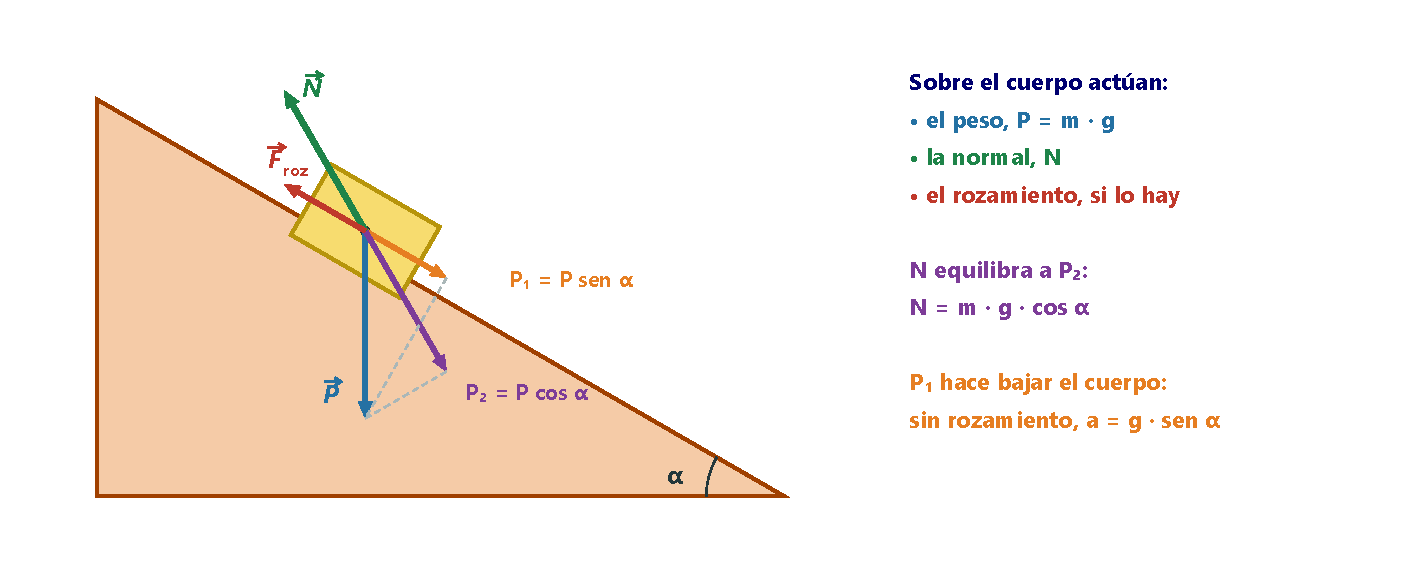
\includegraphics[width=0.8\textwidth]{images/UD10/plano_inclinado}
    \caption{Fuerzas sobre un cuerpo en un plano inclinado y componentes del peso (aquí \(P_1 = P_x\) y \(P_2 = P_y\)).}
    \label{fig:ud11-plano}
\end{figure}

\begin{example}
    \textbf{Un estuche por la mesa.} Una alumna inclina su mesa \(18^\circ\) y empuja hacia abajo, paralelamente a la mesa, su estuche
    de \qty{600}{\g} con una fuerza de \qty{4}{\newton}. Calcula la aceleración del estuche: a) sin rozamiento; b) con \(\mu = \num{0.25}\).

    \textbf{Solución.} Tomamos positivo el sentido hacia abajo del plano. \(P = \num{0.6} \cdot \num{9.8} = \qty{5.88}{\newton}\);
    \(P_x = \num{5.88}\sen 18^\circ = \qty{1.82}{\newton}\); \(P_y = N = \num{5.88}\cos 18^\circ = \qty{5.59}{\newton}\).

    a) \(F + P_x = m\,a \Rightarrow a = \dfrac{4 + \num{1.82}}{\num{0.6}} = \qty{9.70}{\m\per\s\squared}\).

    b) \(F_r = \num{0.25} \cdot \num{5.59} = \qty{1.40}{\newton}\); \(a = \dfrac{4 + \num{1.82} - \num{1.40}}{\num{0.6}} = \qty{7.36}{\m\per\s\squared}\).
\end{example}

\begin{example}
    \textbf{Lanzar hacia arriba por un tobogán.} La misma alumna lanza su estuche hacia arriba por un tobogán inclinado \(25^\circ\),
    con una velocidad de \qty{3}{\m\per\s}. Si \(\mu = \num{0.3}\), ¿qué distancia recorre hasta pararse?

    \textbf{Solución.} Ahora tomamos positivo el sentido del movimiento (hacia arriba). Tanto \(P_x\) como el rozamiento se oponen:
    \(P_x = \num{5.88}\sen 25^\circ = \qty{2.48}{\newton}\); \(N = \num{5.88}\cos 25^\circ = \qty{5.33}{\newton}\); \(F_r = \qty{1.60}{\newton}\).
    \[ -P_x - F_r = m\,a \Rightarrow a = -\frac{\num{2.48} + \num{1.60}}{\num{0.6}} = \qty{-6.81}{\m\per\s\squared} \]
    Con la cinemática: \(v^2 = v_0^2 + 2\,a\,\Delta x \Rightarrow \Delta x = \dfrac{0 - 3^2}{2 \cdot (\num{-6.81})} = \qty{0.66}{\m}\).
\end{example}

\begin{exercise}
    Un camión empieza a verter la leña que transporta cuando la inclinación del volquete llega a \(28^\circ\). ¿Cuál es el
    coeficiente de rozamiento estático entre la leña y el volquete?
    \begin{solu}
        \textcolor{blue}{Justo antes de deslizar, \(m\,g\sen\alpha = \mu_e\,m\,g\cos\alpha\).} \(\mu_e = \tg 28^\circ = \textcolor{red}{\num{0.53}}\).
    \end{solu}
\end{exercise}

\begin{exercise}
    Un bloque de \qty{3}{\kg} está en un plano inclinado \(30^\circ\) y se empuja hacia abajo con una fuerza de \qty{10}{\newton}
    paralela al plano. Calcula su aceleración: a) sin rozamiento; b) con \(\mu = \num{0.25}\).
    \begin{solu}
        \(P_x = \qty{14.7}{\newton}\), \(N = \qty{25.5}{\newton}\). a) \(a = \dfrac{10 + \num{14.7}}{3} = \textcolor{red}{\qty{8.23}{\m\per\s\squared}}\).
        b) \(F_r = \qty{6.37}{\newton}\): \(a = \dfrac{\num{24.7} - \num{6.37}}{3} = \textcolor{red}{\qty{6.11}{\m\per\s\squared}}\).
    \end{solu}
\end{exercise}

\subsection{Cuerpos enlazados}

Muchas veces varios cuerpos se mueven juntos unidos por cuerdas: una grúa que arrastra un coche, los vagones de un tren, una polea con
dos pesas (figura~\ref{fig:ud11-enlazados}). Para resolver estos problemas:

\begin{enumerate}[label=\numberballgreen]
    \item Si las cuerdas son inextensibles y sin masa, la distancia entre los cuerpos no cambia: todos tienen la misma velocidad y la
    misma aceleración en \textbf{módulo}, y la tensión es la misma en toda la cuerda.
    \item Elige un sistema de referencia para cada cuerpo, con el eje \(X\) en la dirección de su movimiento.
    \item Aplica la segunda ley a \textbf{cada cuerpo por separado}, con solo las fuerzas que actúan sobre él. Obtendrás un sistema de
    ecuaciones cuyas incógnitas suelen ser la aceleración y la tensión.
\end{enumerate}

\begin{figure}[H]
    \centering
    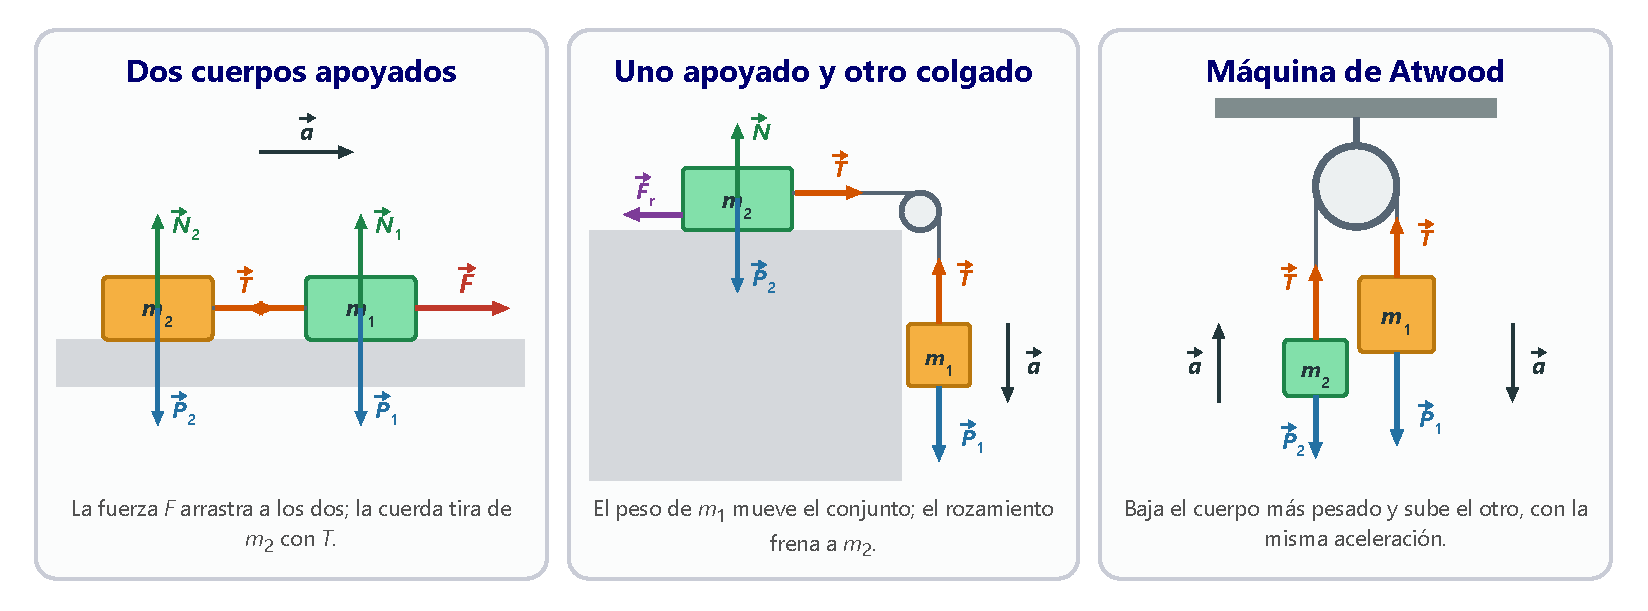
\includegraphics[width=\textwidth]{images/UD11/cuerpos_enlazados}
    \caption{Fuerzas sobre cuerpos enlazados en tres situaciones típicas.}
    \label{fig:ud11-enlazados}
\end{figure}

\begin{remark}
    Si solo queremos la aceleración, podemos tratar el conjunto como un solo cuerpo de masa \(m_1 + m_2\): las tensiones son fuerzas
    interiores y se cancelan. Para calcular la tensión, en cambio, hay que aplicar la segunda ley a uno de los cuerpos.
\end{remark}

\begin{example}
    \textbf{Dos bloques arrastrados.} Dos bloques de \(m_1 = \qty{20}{\kg}\) y \(m_2 = \qty{30}{\kg}\), unidos por una cuerda, se
    arrastran por el suelo sin rozamiento tirando de \(m_1\) con una fuerza horizontal de \qty{400}{\newton}
    (figura~\ref{fig:ud11-enlazados}, izquierda). Calcula la aceleración y la tensión de la cuerda.

    \textbf{Solución.} Sobre el conjunto, la única fuerza horizontal exterior es \(F\):
    \(a = \dfrac{F}{m_1 + m_2} = \dfrac{400}{50} = \qty{8}{\m\per\s\squared}\).
    Sobre \(m_2\) solo tira la cuerda: \(T = m_2\,a = 30 \cdot 8 = \qty{240}{\newton}\). (Comprobación con \(m_1\):
    \(F - T = 400 - 240 = 160 = 20 \cdot 8\).)
\end{example}

\begin{example}
    \textbf{Un bloque en la mesa y otro colgado.} Un cuerpo de \(m_1 = \qty{8}{\kg}\) cuelga de una cuerda que pasa por una polea y
    está unida a otro de \(m_2 = \qty{5}{\kg}\) apoyado en una mesa (figura~\ref{fig:ud11-enlazados}, centro). Si el coeficiente de
    rozamiento entre \(m_2\) y la mesa es \num{0.2}, calcula la aceleración y la tensión.

    \textbf{Solución.} El conjunto se mueve en el sentido en que cae \(m_1\). Ecuaciones de cada cuerpo:
    \[ m_2:\; T - \mu\,m_2\,g = m_2\,a \qquad\qquad m_1:\; m_1\,g - T = m_1\,a \]
    Sumándolas se elimina la tensión:
    \[ a = g\,\frac{m_1 - \mu\,m_2}{m_1 + m_2} = \num{9.8} \cdot \frac{8 - \num{0.2} \cdot 5}{13} = \qty{5.28}{\m\per\s\squared} \]
    Con la ecuación de \(m_1\): \(T = m_1\,(g - a) = 8 \cdot (\num{9.8} - \num{5.28}) = \qty{36.2}{\newton}\).
\end{example}

\paragraph{La máquina de Atwood.} Es una polea con una cuerda de cuyos extremos cuelgan dos cuerpos de masas parecidas
(figura~\ref{fig:ud11-enlazados}, derecha). La inventó George Atwood en 1784 para comprobar las leyes de la dinámica. Si \(m_1 > m_2\),
\(m_1\) baja y \(m_2\) sube con la misma aceleración:
\[ m_1\,g - T = m_1\,a \qquad T - m_2\,g = m_2\,a \qquad\Longrightarrow\qquad a = \frac{m_1 - m_2}{m_1 + m_2}\,g \]
Como la aceleración es mucho menor que \(g\), el movimiento es lento y fácil de medir: es una forma sencilla de medir \(g\).

\begin{exercise}
    Calcula la aceleración y la tensión del ejemplo de los dos bloques arrastrados si el coeficiente de rozamiento con el suelo es
    \num{0.1}.
    \begin{solu}
        \(a = \dfrac{400 - \num{0.1} \cdot 50 \cdot \num{9.8}}{50} = \textcolor{red}{\qty{7.02}{\m\per\s\squared}}\);
        \(T = 30 \cdot \num{7.02} + \num{0.1} \cdot 30 \cdot \num{9.8} = \textcolor{red}{\qty{240}{\newton}}\) (no cambia).
    \end{solu}
\end{exercise}

\begin{exercise}
    En una máquina de Atwood cuelgan dos cuerpos de \qty{6}{\kg} y \qty{9}{\kg}. Determina el sentido del movimiento, la aceleración y
    la tensión de la cuerda.
    \begin{solu}
        \textcolor{red}{Baja el de \qty{9}{\kg}}. \(a = \dfrac{3}{15} \cdot \num{9.8} = \textcolor{red}{\qty{1.96}{\m\per\s\squared}}\);
        \(T = 6 \cdot (\num{9.8} + \num{1.96}) = \textcolor{red}{\qty{70.6}{\newton}}\).
    \end{solu}
\end{exercise}

%========================================================================================
\section{Dinámica del movimiento circular}\label{sec:ud11-circular}
%========================================================================================

El movimiento circular está por todas partes: los satélites que orbitan la Tierra, los huracanes, una atracción de feria o la ropa
en el tambor de una lavadora. En un movimiento circular, la dirección de la velocidad cambia continuamente, así que hay una
\textbf{aceleración normal o centrípeta}, \(\vec{a}_n\), dirigida hacia el centro. Por la segunda ley, tiene que haber una fuerza que
la produzca.

\begin{definition}[Fuerza centrípeta]
    Es la resultante de todas las fuerzas que actúan sobre un cuerpo en la dirección perpendicular a su velocidad. Tiene dirección
    radial, sentido hacia el centro de la circunferencia y módulo
    \[ F_c = m\,a_c = m\,\frac{v^2}{r} = m\,\omega^2\,r \]
\end{definition}

\begin{remark}
    La fuerza centrípeta \textbf{no es una fuerza nueva}, sino el papel que hacen otras: el peso, la tensión de una cuerda, el
    rozamiento, la normal o una combinación de ellas. Si desaparece, el cuerpo sigue en línea recta, tangente a la trayectoria
    (figura~\ref{fig:ud11-centripeta}). La llamada «fuerza centrífuga» solo aparece al describir el movimiento desde un sistema de
    referencia que gira con el cuerpo, que no es inercial.
\end{remark}

\begin{figure}[H]
    \centering
    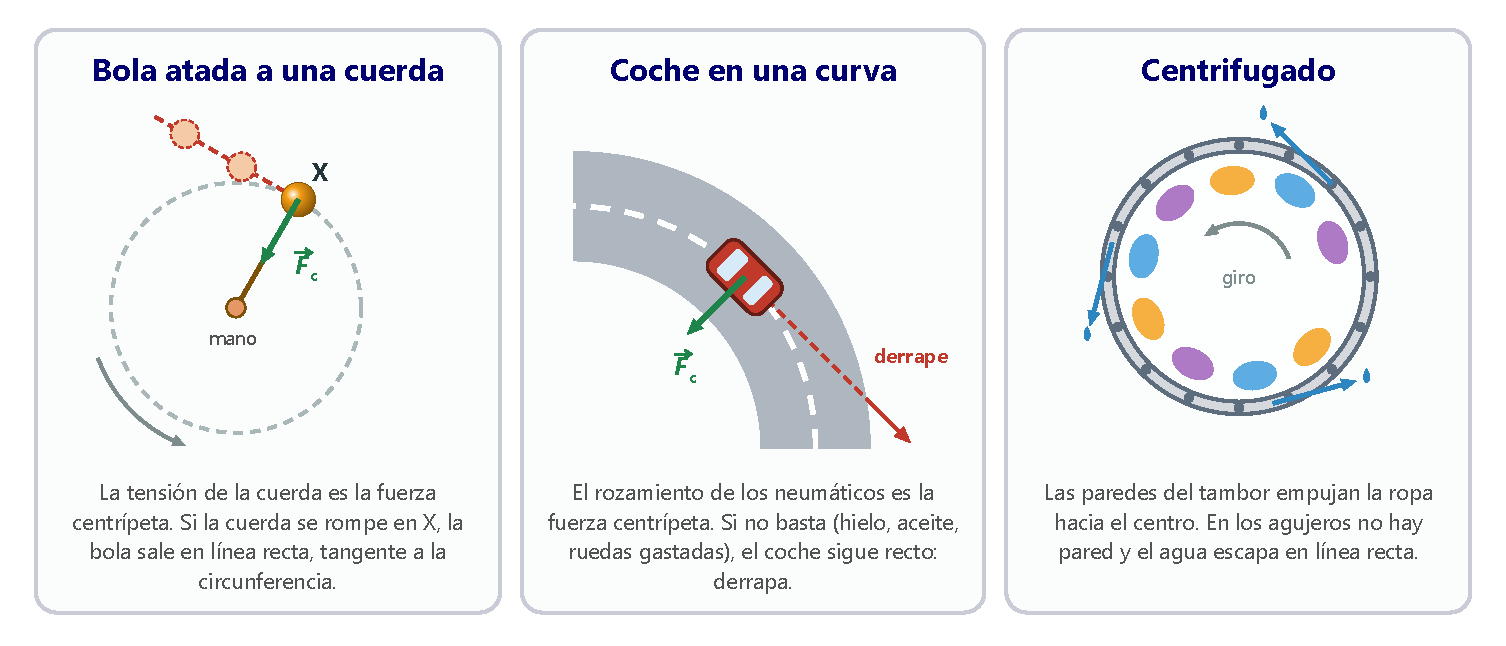
\includegraphics[width=\textwidth]{images/UD11/sin_fuerza_centripeta}
    \caption{Tres ejemplos de fuerza centrípeta y qué ocurre cuando falta.}
    \label{fig:ud11-centripeta}
\end{figure}

\paragraph{MCU y MCUA.} En un \textbf{MCU} el módulo de la velocidad no cambia: no hay aceleración tangencial y la fuerza neta es la
centrípeta, \(\sum\vec{F} = m\,\vec{a}_c\). En un \textbf{MCUA} hay además una aceleración tangencial \(a_t = \alpha\,r\), y la fuerza
neta tiene dos componentes: \(F_c = m\,a_c\) (hacia el centro) y \(F_t = m\,a_t\) (tangente a la trayectoria).

\paragraph{Procedimiento.} 1) Toma un eje radial (hacia el centro) y otro tangente a la trayectoria. 2) Dibuja todas las fuerzas, la
velocidad y la aceleración centrípeta. 3) Aplica la segunda ley en la dirección radial: \(\sum F_{\text{radial}} = m\,v^2/r\). Recuerda
las relaciones de la cinemática: \(v = \omega\,r\), \(\omega = 2\pi/T = 2\pi f\).

\begin{example}
    \textbf{Centrifugar la ropa.} El tambor de una lavadora tiene \qty{50}{\cm} de diámetro y centrifuga a \qty{1200}{rpm}. ¿Qué
    fuerza centrípeta actúa sobre \qty{7}{\kg} de ropa pegada a la pared del tambor?

    \textbf{Solución.} \(\omega = 1200 \cdot \dfrac{2\pi}{60} = \qty{125.7}{\radian\per\s}\);
    \(a_c = \omega^2\,r = \num{125.7}^2 \cdot \num{0.25} = \qty{3.95e3}{\m\per\s\squared}\), unas 400 veces \(g\).
    \(F_c = 7 \cdot \num{3.95e3} = \qty{2.8e4}{\newton}\). La hace la pared del tambor; el agua, que pasa por los agujeros, no recibe
    esa fuerza y sale en línea recta.
\end{example}

\begin{example}
    \textbf{En una rotonda.} Un coche de \qty{1200}{\kg} toma una rotonda de \qty{40}{\m} de radio a \qty{30}{\km\per\hour}. Calcula
    su aceleración centrípeta y la fuerza centrípeta.

    \textbf{Solución.} \(v = \qty{8.33}{\m\per\s}\); \(a_c = \dfrac{\num{8.33}^2}{40} = \qty{1.74}{\m\per\s\squared}\);
    \(F_c = 1200 \cdot \num{1.74} = \qty{2083}{\newton}\). Esta fuerza la hace el rozamiento entre los neumáticos y el asfalto.
\end{example}

\subsection{El movimiento de los satélites}

En una primera aproximación, un satélite describe una órbita circular de radio \(r\) (la distancia al centro del planeta) con
velocidad constante. La fuerza centrípeta es la atracción gravitatoria del planeta:
\[ G\,\frac{M\,m}{r^2} = m\,\frac{v^2}{r} \quad\Longrightarrow\quad v = \sqrt{\frac{G\,M}{r}} \qquad T = \frac{2\pi r}{v} = 2\pi\sqrt{\frac{r^3}{G\,M}} \]
La velocidad no depende de la masa del satélite, y cuanto más alta es la órbita, más despacio va y más tarda en dar una vuelta
(figura~\ref{fig:ud11-orbitas}).

\begin{figure}[H]
    \centering
    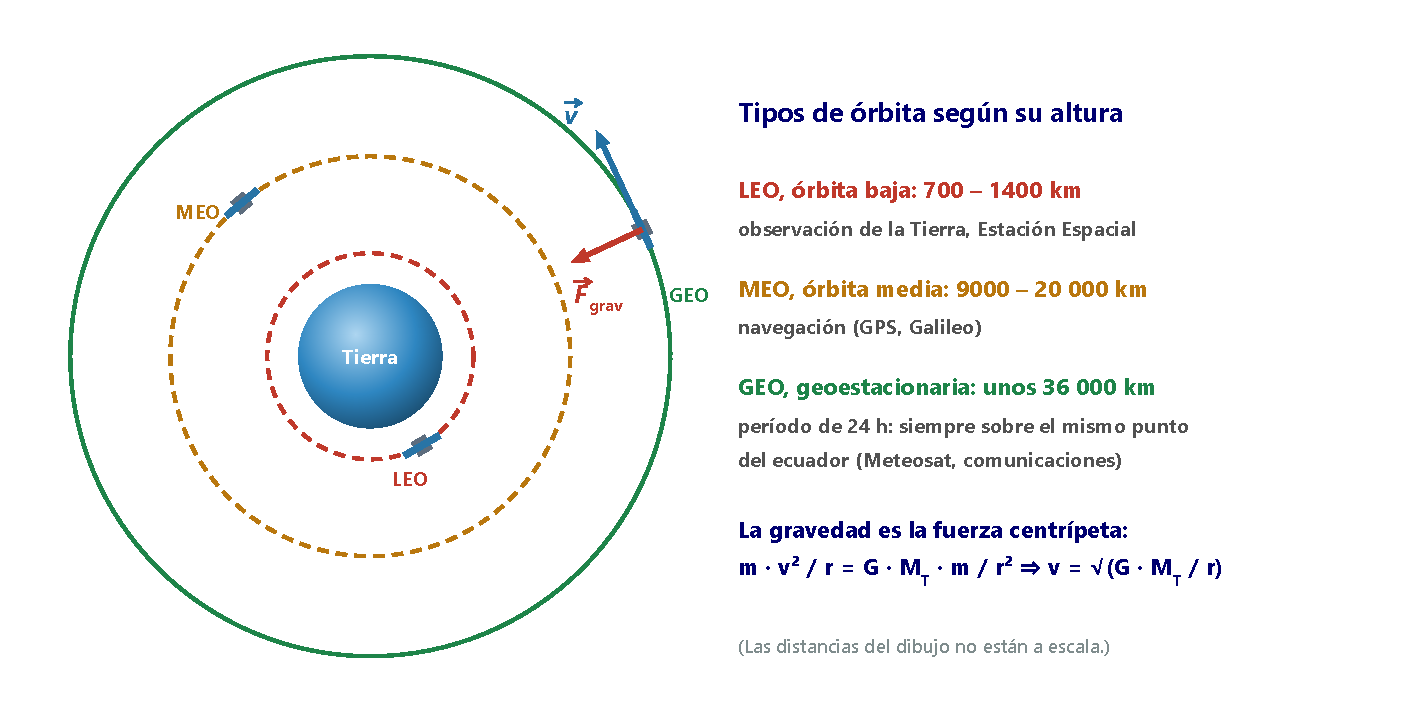
\includegraphics[width=0.8\textwidth]{images/UD11/orbitas_satelites}
    \caption{Órbitas bajas, medias y geoestacionarias. La gravedad es la fuerza centrípeta.}
    \label{fig:ud11-orbitas}
\end{figure}

\begin{example}
    \textbf{Un satélite de observación.} Calcula la velocidad y el periodo de un satélite que orbita a \qty{700}{\km} de altura.

    \textbf{Solución.} \(r = 6370 + 700 = \qty{7070}{\km}\).
    \[ v = \sqrt{\frac{\num{6.67e-11} \cdot \num{5.97e24}}{\num{7.07e6}}} = \qty{7.50e3}{\m\per\s} \qquad
    T = \frac{2\pi \cdot \num{7.07e6}}{\num{7.50e3}} = \qty{5.92e3}{\s} \approx \qty{99}{\minute} \]
\end{example}

\subsection{Coches en las curvas}

\paragraph{Curva plana.} El coche describe un arco de circunferencia y la única fuerza horizontal es el \textbf{rozamiento} lateral
entre los neumáticos y el asfalto, que hace de fuerza centrípeta; en vertical, el peso y la normal se equilibran
(figura~\ref{fig:ud11-curvas}). La velocidad máxima sin derrapar se alcanza cuando el rozamiento llega a su valor máximo:
\[ \mu\,m\,g = m\,\frac{v^2}{r} \quad\Longrightarrow\quad v_{\text{máx}} = \sqrt{\mu\,g\,r} \]

\paragraph{Curva peraltada.} Si la carretera está inclinada hacia el interior un ángulo \(\alpha\) (peralte), la normal tiene una
componente horizontal que contribuye a la fuerza centrípeta. Sin rozamiento:
\[ N\cos\alpha = m\,g \qquad N\sen\alpha = m\,\frac{v^2}{r} \quad\Longrightarrow\quad v = \sqrt{g\,r\tg\alpha} \]

\begin{figure}[H]
    \centering
    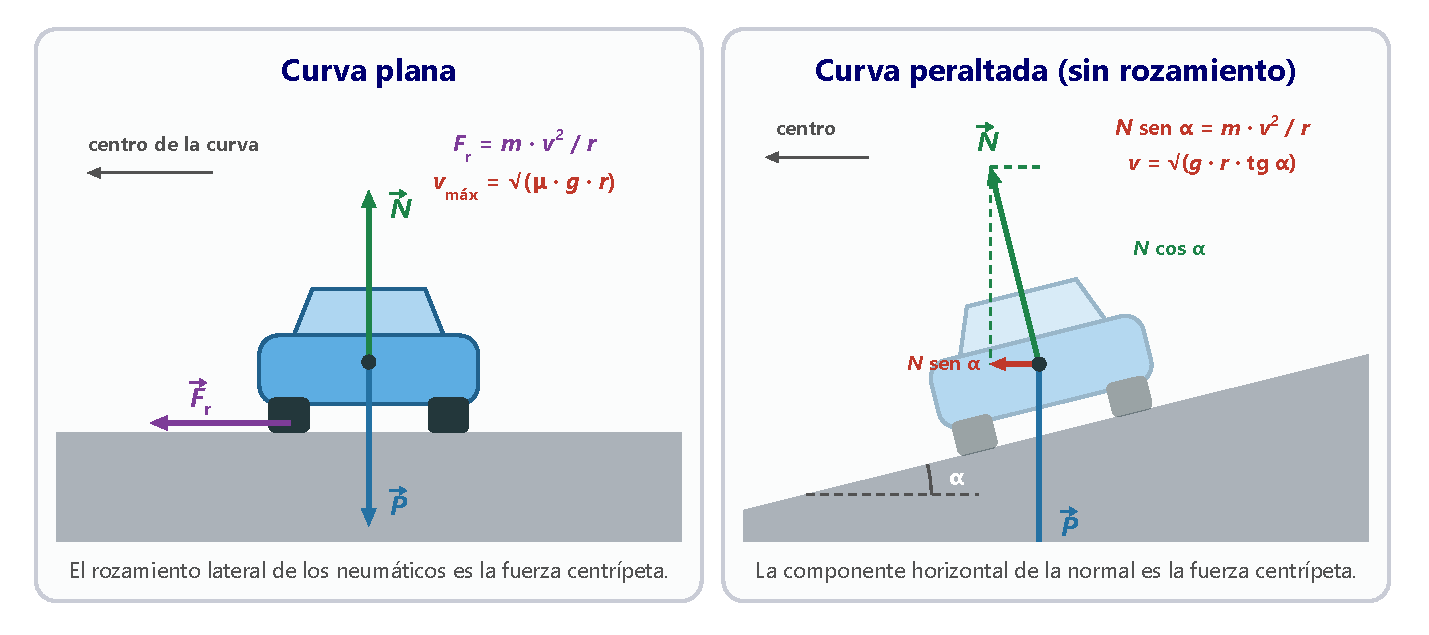
\includegraphics[width=0.95\textwidth]{images/UD11/curvas}
    \caption{Fuerzas sobre un coche en una curva plana y en una curva peraltada.}
    \label{fig:ud11-curvas}
\end{figure}

\begin{remark}
    La velocidad máxima en una curva no depende de la masa del vehículo, sino del radio y del coeficiente de rozamiento, que cambia
    mucho con el estado del asfalto y de los neumáticos (presión, desgaste) o si hay agua o hielo.
\end{remark}

\begin{example}
    \textbf{Velocidad máxima en una curva.} Una curva tiene \qty{80}{\m} de radio. Calcula la velocidad máxima: a) si es plana y el
    coeficiente de rozamiento es \num{0.6}; b) si tiene un peralte de \(10^\circ\) y no hubiera rozamiento (hielo).

    \textbf{Solución.} a) \(v = \sqrt{\num{0.6} \cdot \num{9.8} \cdot 80} = \qty{21.7}{\m\per\s}\) (\qty{78}{\km\per\hour}).
    b) \(v = \sqrt{\num{9.8} \cdot 80 \cdot \tg 10^\circ} = \qty{11.8}{\m\per\s}\) (\qty{42}{\km\per\hour}).
\end{example}

\begin{exercise}
    Un patinador de \qty{70}{\kg} recorre un circuito circular de \qty{20}{\m} de radio y está sometido a una fuerza centrípeta de
    \qty{315}{\newton}. ¿Qué velocidad lleva?
    \begin{solu}
        \(v = \sqrt{\dfrac{F_c\,r}{m}} = \sqrt{\dfrac{315 \cdot 20}{70}} = \textcolor{red}{\qty{9.49}{\m\per\s}}\).
    \end{solu}
\end{exercise}

\begin{exercise}
    Un coche teledirigido de \qty{2}{\kg} da 6 vueltas por minuto en una pista circular de \qty{1.5}{\m} de radio. ¿Qué fuerza
    centrípeta actúa sobre él?
    \begin{solu}
        \(\omega = \dfrac{6 \cdot 2\pi}{60} = \qty{0.628}{\radian\per\s}\); \(F_c = 2 \cdot \num{0.628}^2 \cdot \num{1.5} = \textcolor{red}{\qty{1.18}{\newton}}\).
    \end{solu}
\end{exercise}

\begin{exercise}
    Un cuerpo de \qty{4}{\kg} gira con MCU en una circunferencia de \qty{50}{\cm} de radio sometido a una fuerza centrípeta de
    \qty{120}{\newton}. ¿Cuánto tarda en dar una vuelta?
    \begin{solu}
        \(\omega = \sqrt{\dfrac{120}{4 \cdot \num{0.5}}} = \qty{7.75}{\radian\per\s}\); \(T = \dfrac{2\pi}{\omega} = \textcolor{red}{\qty{0.81}{\s}}\).
    \end{solu}
\end{exercise}

\begin{exercise}
    Un satélite meteorológico de \qty{2000}{\kg} está en órbita geoestacionaria, a \qty{42164}{\km} del centro de la Tierra. Calcula su
    velocidad y la fuerza centrípeta a la que está sometido.
    \begin{solu}
        \(v = \sqrt{\dfrac{G\,M_T}{r}} = \textcolor{red}{\qty{3.07e3}{\m\per\s}}\); \(F_c = \dfrac{m\,v^2}{r} = \textcolor{red}{\qty{448}{\newton}}\).
    \end{solu}
\end{exercise}

%========================================================================================
\section{Física en la vida: ¿se cumplen las leyes de la física en el cine?}\label{sec:ud11-cine}
%========================================================================================

Muchas películas de ciencia ficción son un buen laboratorio para poner a prueba lo que sabemos de dinámica.

En las batallas espaciales de muchas sagas, las naves giran inclinándose como aviones y las explosiones se oyen con estruendo. Pero en
el vacío no hay aire: el sonido no se propaga y una nave no puede «apoyarse» en el aire para girar; necesita expulsar gases en la
dirección contraria a la que quiere ir (tercera ley de Newton). Tampoco necesita mantener los motores encendidos para avanzar: por el
principio de inercia, seguiría moviéndose sin ellos.

Las películas de superhéroes ofrecen otro ejemplo clásico: el héroe atrapa en el aire a una persona que cae desde un rascacielos y la
detiene en un instante. Pero, por el teorema del impulso, frenar a una persona en muy poco tiempo exige una fuerza enorme: el «rescate»
sería tan dañino como el choque contra el suelo.

En cambio, \textit{Interstellar} (2014) contó con el asesoramiento del físico Kip Thorne, premio Nobel en 2017 por la detección de las
ondas gravitacionales. Su imagen del agujero negro Gargantúa se calculó con las ecuaciones de la relatividad general y resultó muy
parecida a la primera imagen real de un agujero negro, obtenida en 2019. El cine también puede ser una forma estupenda de divulgar la
ciencia.

\begin{exercise}
    a) Un superhéroe atrapa a una persona de \qty{60}{\kg} que cae a \qty{30}{\m\per\s} y la detiene en \qty{0.05}{\s}. ¿Qué fuerza media
    sufre la persona? ¿Cuántas veces su peso? ¿Y si la frenara en \qty{1}{\s}? b) En una película, una nave espacial gira en el vacío
    describiendo una curva cerrada con los motores apagados. ¿Es posible? c) Elegid una escena de una película y analizad si respeta las
    leyes de la dinámica.
    \begin{solu}
        a) \(F = \dfrac{60 \cdot 30}{\num{0.05}} = \textcolor{red}{\qty{3.6e4}{\newton}}\), unas \textcolor{red}{61 veces su peso}; en
        \qty{1}{\s}, \textcolor{red}{\qty{1800}{\newton}} (unas 3 veces su peso). b) \textcolor{red}{No}: para describir una curva hace
        falta una fuerza centrípeta; sin motores (y lejos de cualquier astro) la nave seguiría en línea recta. c) \textcolor{red}{Respuesta
        abierta}.
    \end{solu}
\end{exercise}

%========================================================================================
\section{Prácticas}\label{sec:ud11-practicas}
%========================================================================================

\subsection{El coeficiente de rozamiento estático con un libro}

\noindent\begin{minipage}[t]{0.48\textwidth}
    \textbf{Objetivo}
    \begin{itemize}
        \item Medir el coeficiente de rozamiento estático entre distintos objetos y la tapa de un libro.
    \end{itemize}
\end{minipage}\hfill
\begin{minipage}[t]{0.48\textwidth}
    \textbf{Material}
    \begin{itemize}
        \item Un libro grande de tapa dura, una regla, una moneda, un móvil (con y sin funda) y otros objetos pequeños.
    \end{itemize}
\end{minipage}

\begin{figure}[H]
    \centering
    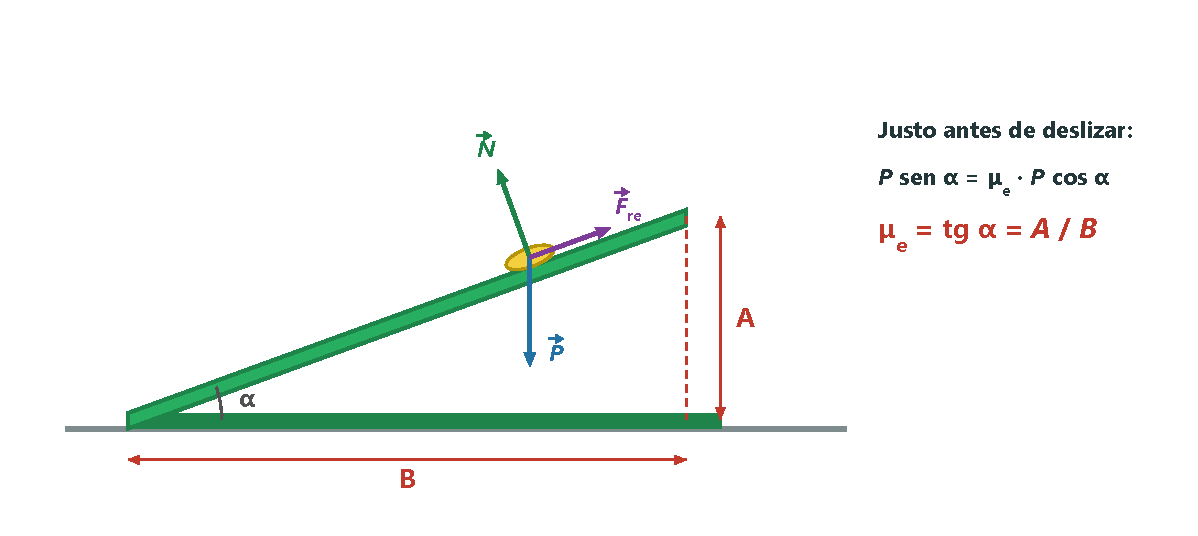
\includegraphics[width=0.75\textwidth]{images/UD11/practica_libro}
    \caption{Se levanta la tapa del libro hasta que el objeto empieza a deslizar.}
    \label{fig:ud11-libro}
\end{figure}

\textbf{Procedimiento}
\begin{enumerate}[label=\numberballgreen]
    \item Coloca el libro cerrado sobre la mesa y pon la moneda cerca del borde superior de la tapa.
    \item Levanta poco a poco la tapa hasta que la moneda empiece a deslizar. En ese momento, mide la altura \(A\) del borde de la tapa y
    la distancia horizontal \(B\) desde el lomo hasta la vertical de ese borde.
    \item Repite la medida tres veces y calcula la media. Haz lo mismo con los demás objetos.
\end{enumerate}

\begin{exercise}
    a) Demuestra que, justo cuando el objeto empieza a deslizar, \(\mu_e = \tg\alpha = A/B\). b) Con la moneda, un grupo mide
    \(A = \qty{6.2}{\cm}\) y \(B = \qty{21.0}{\cm}\); con el móvil en su funda de goma, \(A = \qty{12.8}{\cm}\) y \(B = \qty{17.5}{\cm}\).
    Calcula los coeficientes y el ángulo en el caso de la moneda. c) ¿Influye la masa del objeto? ¿Y el tamaño de la superficie de
    contacto?
    \begin{solu}
        a) \textcolor{blue}{En el límite, \(m\,g\sen\alpha = \mu_e\,m\,g\cos\alpha\).} \(\textcolor{red}{\mu_e = \tg\alpha}\), y
        \(\tg\alpha = A/B\). b) Moneda: \(\mu_e = \textcolor{red}{\num{0.30}}\) (\(\alpha = \textcolor{red}{\num{16.4}^\circ}\));
        móvil: \(\mu_e = \textcolor{red}{\num{0.73}}\). c) \textcolor{red}{No}: la masa se simplifica, y el coeficiente apenas depende del
        área de contacto; \textcolor{red}{depende de los materiales} y de lo rugosos que sean.
    \end{solu}
\end{exercise}

\subsection{Medir \texorpdfstring{\(g\)}{g} con una máquina de Atwood}

\noindent\begin{minipage}[t]{0.48\textwidth}
    \textbf{Objetivo}
    \begin{itemize}
        \item Construir una máquina de Atwood y usarla para medir la aceleración de la gravedad.
    \end{itemize}
\end{minipage}\hfill
\begin{minipage}[t]{0.48\textwidth}
    \textbf{Material}
    \begin{itemize}
        \item Una polea ligera (o el carrete de una caña de pescar), hilo resistente, dos vasos de plástico, arena o monedas, una
        balanza, una cinta métrica y un cronómetro.
    \end{itemize}
\end{minipage}

\textbf{Procedimiento}
\begin{enumerate}[label=\numberballgreen]
    \item Sujeta la polea a un soporte alto, pasa el hilo por ella y ata un vaso en cada extremo.
    \item Llena los vasos con arena hasta que tengan masas un poco distintas (por ejemplo, \qty{260}{\g} y \qty{240}{\g}).
    \item Coloca el vaso más pesado a \qty{1}{\m} del suelo, suéltalo desde el reposo y mide el tiempo que tarda en llegar al suelo.
    Repite cinco veces y calcula la media.
\end{enumerate}

\begin{exercise}
    a) Demuestra que \(g = a\,\dfrac{m_1 + m_2}{m_1 - m_2}\), con \(a = 2d/t^2\). b) Con \(m_1 = \qty{260}{\g}\), \(m_2 = \qty{240}{\g}\) y
    \(d = \qty{1.00}{\m}\), el tiempo medio es de \qty{2.27}{\s}. Calcula \(g\) y el error relativo respecto a \qty{9.8}{\m\per\s\squared}.
    c) ¿Por qué conviene que las masas sean parecidas? ¿Qué factores no hemos tenido en cuenta?
    \begin{solu}
        a) Despejando \(g\) de \(a = \dfrac{m_1 - m_2}{m_1 + m_2}\,g\). b) \(a = \dfrac{2}{\num{2.27}^2} = \qty{0.388}{\m\per\s\squared}\);
        \(g = \num{0.388} \cdot \dfrac{500}{20} = \textcolor{red}{\qty{9.70}{\m\per\s\squared}}\); error relativo \(\textcolor{red}{\qty{1}{\percent}}\).
        c) \textcolor{red}{Para que la aceleración sea pequeña y el tiempo, fácil de medir.} No hemos tenido en cuenta el
        \textcolor{red}{rozamiento de la polea, su masa ni la del hilo}.
    \end{solu}
\end{exercise}

%========================================================================================
\section{Situación de aprendizaje: satélites al servicio del planeta (ODS 17)}\label{sec:ud11-ods}
%========================================================================================

Desde que la Unión Soviética lanzó el \textbf{Sputnik 1} el 4 de octubre de 1957, el primer satélite artificial, miles de satélites
orbitan la Tierra. Hoy dependemos de ellos para las comunicaciones, la navegación por GPS y Galileo, la predicción meteorológica, la
vigilancia del medio ambiente o la respuesta ante catástrofes. Según la ONU, los datos de observación de la Tierra ayudan a cumplir
muchas de las metas de los Objetivos de Desarrollo Sostenible: permiten medir el cambio climático, detectar la contaminación del aire y
del agua o mejorar la agricultura.

La exploración del espacio es también un ejemplo del \textbf{ODS 17} (alianzas para lograr los objetivos): la Estación Espacial
Internacional es fruto de la colaboración de las agencias de Estados Unidos, Rusia, Europa, Japón y Canadá, y la Oficina de Asuntos del
Espacio Ultraterrestre de la ONU (UNOOSA) promueve el uso pacífico del espacio y lleva el registro de los objetos lanzados, para
evitar acumular más basura espacial.

\begin{marker}
    \textbf{Reto:} por grupos, preparad un mural o una presentación sobre una misión espacial europea (por ejemplo, Galileo, Copernicus,
    Meteosat de Tercera Generación o Rosetta): para qué sirve, qué órbita sigue y qué física hay detrás.
\end{marker}

\begin{enumerate}[label=\numberballred]
    \item \textbf{Investigad} qué es una órbita baja, una órbita media y una órbita geoestacionaria, y qué tipo de satélites usa cada una.
    \item \textbf{Calculad} la altura de la órbita geoestacionaria (periodo de un día sidéreo, \qty{86164}{\s}) y el periodo de la
    Estación Espacial, a \qty{420}{\km} de altura.
    \item \textbf{Analizad} el problema de la basura espacial: ¿por qué los restos se quedan en órbita durante años?
    \item \textbf{Comunicad} vuestro trabajo explicando cómo ayudan los satélites a lograr al menos tres ODS.
\end{enumerate}

\begin{exercise}
    Resuelve el apartado 2 de la situación de aprendizaje. ¿A qué velocidad se mueve un satélite geoestacionario?
    \begin{solu}
        \textcolor{blue}{De \(T = 2\pi\sqrt{r^3/(G\,M_T)}\):} \(r = \sqrt[3]{\dfrac{G\,M_T\,T^2}{4\pi^2}} = \textcolor{red}{\qty{4.22e7}{\m}}\),
        es decir, a unos \textcolor{red}{\qty{35800}{\km}} de altura; \(v = \dfrac{2\pi r}{T} = \textcolor{red}{\qty{3.07}{\km\per\s}}\).
        Estación Espacial: \(r = \qty{6.79e6}{\m}\), \(T = \textcolor{red}{\qty{92.9}{\minute}}\).
    \end{solu}
\end{exercise}
